\documentclass[12pt]{article}

\usepackage{amsmath}
\usepackage{booktabs}
\usepackage{graphicx}
\usepackage[numbers]{natbib}
\usepackage{hyperref}
\usepackage[margin=1in]{geometry}
\usepackage{setspace}
\doublespacing

\title{\textbf{Transfer Learning from Lithium-Ion to Zinc-Ion Batteries:\\
Cross-Chemistry Capacity Prediction with Limited Target Data}}

\author{Xueyang Song}

\date{2026}

\begin{document}

\maketitle

\begin{abstract}
Zinc-ion batteries (ZIBs) are emerging as a low-cost, safe alternative to
lithium-ion batteries (LIBs) for grid-scale energy storage, but their data
scarcity makes accurate lifetime prediction challenging. We investigate whether
degradation knowledge from data-rich LIB datasets (Severson/MATR: 124 cells;
CALCE: 8 cells) can be transferred to improve capacity prediction for ZIBs under
limited data regimes ($N = 2$--$40$ training cells). We propose a Selective
Multi-Task Gaussian Process (Selective MT-GP) that explicitly partitions features
by transferability: the exponential decay rate ($\text{exp\_b}$) is shared across
both chemistries via an inter-task kernel, while the differential capacity
variance ($\Delta\mathrm{var}(dQ/dV)$) --- which exhibits a 1000-fold absolute
scale gap between chemistries --- is treated as a Zn-ion-private feature.

Our experiments reveal a critical crossover at $N \approx 20$: below this
threshold, Li-ion labels actively harm Zn-ion predictions (negative transfer),
while above it, selective feature transfer outperforms na\"ive approaches.
Crucially, while Selective MT-GP does not achieve lower RMSE than a direct
Zn-ion GP (GP-Direct), it provides dramatically better-calibrated uncertainty
estimates at small $N$: at $N = 2$, GP-Direct achieves only 50.5\% coverage of
its stated 90\% credible intervals ($\mathrm{NLL} = 3.44$), compared to 81\%
coverage for Selective MT-GP ($\mathrm{NLL} = 1.07$ --- a 3.2$\times$
improvement). These results establish that cross-chemistry transfer learning's
primary value lies in uncertainty calibration rather than point accuracy, with
implications for safe deployment in new-chemistry battery development.
\end{abstract}

% ============================================================
\section{Introduction}
\label{sec:intro}
% ============================================================

The global transition to renewable energy demands large-scale, cost-effective,
and safe stationary energy storage. Zinc-ion batteries have attracted intense
interest as next-generation grid-storage devices, offering several compelling
advantages over conventional lithium-ion technology: zinc metal anodes operate
stably in mild aqueous electrolytes (typically ZnSO$_4$ solution), elemental
zinc is earth-abundant and inexpensive, and the absence of organic solvents
eliminates the fire and toxicity hazards inherent in conventional LIBs
\cite{tan2024}. Despite rapid advances in ZIB electrode materials and
electrolyte engineering --- including machine learning-guided interfacial
coating optimization \cite{song2026ald} --- practical deployment at grid scale
still requires reliable lifetime estimation --- the ability to predict remaining useful life
(RUL) or total cycle life from early-cycle measurements so that battery
management systems can schedule maintenance, warranty pricing, and second-life
allocation.

A fundamental obstacle to accurate lifetime modeling for ZIBs is data
scarcity. While the lithium-ion community has accumulated thousands of
well-characterized cell trajectories across diverse chemistries, formats, and
cycling protocols \cite{severson2019, paulson2022}, ZIB lifecycle datasets
remain sparse: the largest publicly available collection contains on the order
of hundreds of cells, and most laboratory studies report far fewer. Machine
learning models trained on such limited data suffer from high variance and
poorly calibrated uncertainty --- a dangerous combination when predictions
inform safety-critical deployment decisions.

A natural hypothesis is that lifetime prediction knowledge can be transferred
from data-rich LIBs to data-scarce ZIBs. Both battery chemistries degrade
monotonically over cycling; at the macroscopic level both exhibit
approximately exponential capacity fade, suggesting that at least some
predictive features may encode universal electrochemical degradation physics
rather than chemistry-specific mechanisms. Multi-task Gaussian processes
\cite{bonilla2007} provide a principled Bayesian framework for such transfer:
by modeling LIB and ZIB lifetime prediction as related tasks sharing a common
latent structure, the model can regularize ZIB predictions using LIB data when
the tasks are positively correlated.

However, this attractive hypothesis conceals two failure modes that we
discover and characterize in this work. \textbf{Failure Mode 1} (normalization
artifact): applying per-domain feature normalization before constructing the
joint model creates a spurious anti-correlation between tasks. Zinc-ion cells
whose differential capacity variance $\Delta\mathrm{var}(dQ/dV)$ is moderate
in absolute terms appear as outliers in the raw feature space but become
``typical'' after per-domain standardization. Because high $\Delta\mathrm{var}$
correlates with short life in the LIB dataset, the standardization maps ZIB
cells to the high-variance LIB regime, inducing a negative inter-task
correlation ($\rho = -0.47$) and degrading ZIB predictions. \textbf{Failure
Mode 2} (feature starvation): even after applying a global log-transform to
compress the ${\sim}1000{\times}$ scale gap in $\Delta\mathrm{var}$ between
LIBs and ZIBs, naive full feature sharing causes the GP's effective length
scales to be dominated by the LIB feature distribution, starving the model of
discriminative power in the ZIB regime.

Our key contribution is the \textbf{Selective Multi-Task Gaussian Process}
(Selective MT-GP), which resolves both failure modes through explicit physical
feature partitioning. The exponential decay rate $\text{exp\_b}$ --- a
parameter reflecting universal macroscopic degradation kinetics analogous to an
Arrhenius activation --- is shared across chemistries via a standard inter-task
coregionalization kernel. The differential capacity variance
$\Delta\mathrm{var}(dQ/dV)$ --- which encodes chemistry-specific phase
transition thermodynamics (LiFePO$_4$ two-phase reaction versus Zn
plating/stripping) and therefore cannot be assumed transferable --- is
restricted to a Zn-ion-private kernel that contributes to ZIB predictions only.

Through systematic Monte Carlo evaluation over $N \in \{2, 5, 10, 20, 40\}$
Zn-ion training cells, we establish a \textbf{critical crossover at
$N \approx 20$}: below this threshold, Li-ion labels actively harm ZIB point
predictions (negative transfer), while above it, selective transfer yields
statistically significant RMSE reductions relative to naive full-sharing.
However, a more practically important finding emerges from our uncertainty
calibration analysis: at $N = 2$, Selective MT-GP reduces the negative
log-likelihood (NLL) by a factor of 3.2$\times$ relative to GP-Direct (from
$\mathrm{NLL} = 3.44$ to $\mathrm{NLL} = 1.07$), and achieves 81\% coverage
versus 50.5\% for GP-Direct's nominally 90\% credible intervals. This
calibration advantage persists until approximately $N = 40$, where both models
converge to well-calibrated predictions with sufficient data.

This paper is organized as follows. Section~\ref{sec:data} describes both the
Li-ion source datasets and the Zn-ion target dataset, along with feature
engineering. Section~\ref{sec:methods} presents the Selective MT-GP
architecture and the evaluation protocol. Section~\ref{sec:results} reports
experimental results, and Section~\ref{sec:discussion} interprets the findings
and discusses engineering implications. Section~\ref{sec:conclusion} concludes.

% ============================================================
\section{Data}
\label{sec:data}
% ============================================================

\subsection{Li-ion Source Data}

Our primary Li-ion source dataset is the Severson/MATR dataset \cite{severson2019},
which comprises 124 LFP (LiFePO$_4$/graphite) pouch cells cycled under diverse
fast-charging policies at room temperature. This dataset is publicly available at
the \texttt{petermattia/revisit-severson-et-al} GitHub repository and is the
standard benchmark for early-cycle battery lifetime prediction. Each cell was
cycled to 80\% capacity retention, providing ground-truth cycle life spanning
roughly 150--2300 cycles.

We supplement this with the CALCE dataset, which contributes 8 additional
LFP/NMC cells cycled under constant-current protocols. After applying a joint
quality filter ($\text{exp\_b} < 4.9$ AND cycle life $> 10$), we retain a
total of 132 Li-ion cells. The filter on $\text{exp\_b}$ removes cells with
anomalously rapid early degradation that is inconsistent with the exponential
decay model (these cells exhibit abrupt capacity plunges likely caused by
manufacturing defects rather than normal aging). The cycle life floor
($> 10$ cycles) ensures that sufficient cycles are available for reliable
feature extraction.

The resulting Li-ion feature ranges after filtering are: $\text{exp\_b} \in
[0, 4.9]$ and $\Delta\mathrm{var}(dQ/dV) \in [0, 11.83]$. These ranges define
the support of the source domain and play a critical role in understanding the
cross-domain scale gap discussed below.

\subsection{Zn-ion Target Data}

The Zn-ion target data are drawn from the BatteryLife dataset \cite{tan2024}
(Zenodo DOI: \href{https://doi.org/10.5281/zenodo.7771988}{10.5281/zenodo.7771988}).
We use the ZN-coin cell subset (Batches 1--3), which consists of coin-cell format
Zn/MnO$_2$ cells cycled in mild aqueous ZnSO$_4$ electrolyte at various
C-rates. After filtering to retain cells with cycle life $\geq 5$, we obtain
100 Zn-ion cells for analysis.

A critical preprocessing step unique to ZIB data is activation cycle removal.
Zinc-ion cells commonly exhibit a capacity \emph{increase} in the first
10--50 cycles as the MnO$_2$ cathode undergoes electrochemical activation
(dissolution/re-deposition of Mn species forms a more electrochemically
accessible structure). Including activation cycles in lifetime model training
introduces a systematic upward bias in early-cycle capacity measurements that is
absent in LIB data. We apply PELT change-point detection \cite{truong2020} to
each cell's capacity trajectory to identify the end of the activation plateau,
and all feature extraction is performed exclusively on post-activation cycles.

After this preprocessing, the Zn-ion $\Delta\mathrm{var}(dQ/dV)$ range is
$[0, 0.011]$ --- approximately $\mathbf{1000\times}$ smaller than the LIB
range of $[0, 11.83]$. This scale gap is the central challenge motivating our
feature engineering strategy.

\subsection{Feature Engineering}

We extract two features per cell from early-cycle data (first 20
post-activation cycles).

\paragraph{Exponential decay rate ($\text{exp\_b}$).}
We fit the following phenomenological model to the normalized capacity trajectory:
\begin{equation}
  \frac{Q(n)}{Q_0} = A + (1 - A)\,\exp(-bn),
  \label{eq:exp_decay}
\end{equation}
where $Q(n)$ is the discharge capacity at cycle $n$, $Q_0$ is the nominal
capacity, $A$ is the asymptotic fractional capacity, and $b > 0$ is the
exponential decay rate. The parameter $b$ captures the rate at which the cell
approaches its long-term plateau and serves as a proxy for the overall
degradation kinetics. Fitting is performed via nonlinear least squares using
cycles 1--20 post-activation; $b$ is the extracted feature.

\paragraph{Differential capacity variance ($\Delta\mathrm{var}(dQ/dV)$).}
For each cycle, we compute the capacity differential $dQ/dV$ using a
Savitzky-Golay filter (window = 11 points, polynomial order = 3) applied to
the voltage-capacity curve. We then compute the cycle-to-cycle variance of the
smoothed $dQ/dV$ profile over the first 20 post-activation cycles. This feature
captures variability in the electrochemical phase transitions: stable phase
transitions (low variance) indicate a well-formed electrode structure and are
associated with longer cell life.

\paragraph{Log-transform and joint scaling.}
To address the 1000$\times$ scale gap in $\Delta\mathrm{var}(dQ/dV)$ between
LIBs and ZIBs, we apply a log-transform:
\begin{equation}
  x_{\log} = \log_{10}\!\bigl(\Delta\mathrm{var}(dQ/dV) + 10^{-6}\bigr).
  \label{eq:logtransform}
\end{equation}
The small constant $10^{-6}$ prevents numerical issues for cells with near-zero
variance. After log-transformation, a \texttt{StandardScaler} is fit jointly
over the combined Li-ion and Zn-ion feature matrix so that both tasks share a
common scale in the model's input space. Figure~\ref{fig:features} shows the
resulting feature distributions, confirming that the log-transform substantially
improves overlap between the LIB and ZIB marginal distributions.

\begin{figure}[htbp]
  \centering
  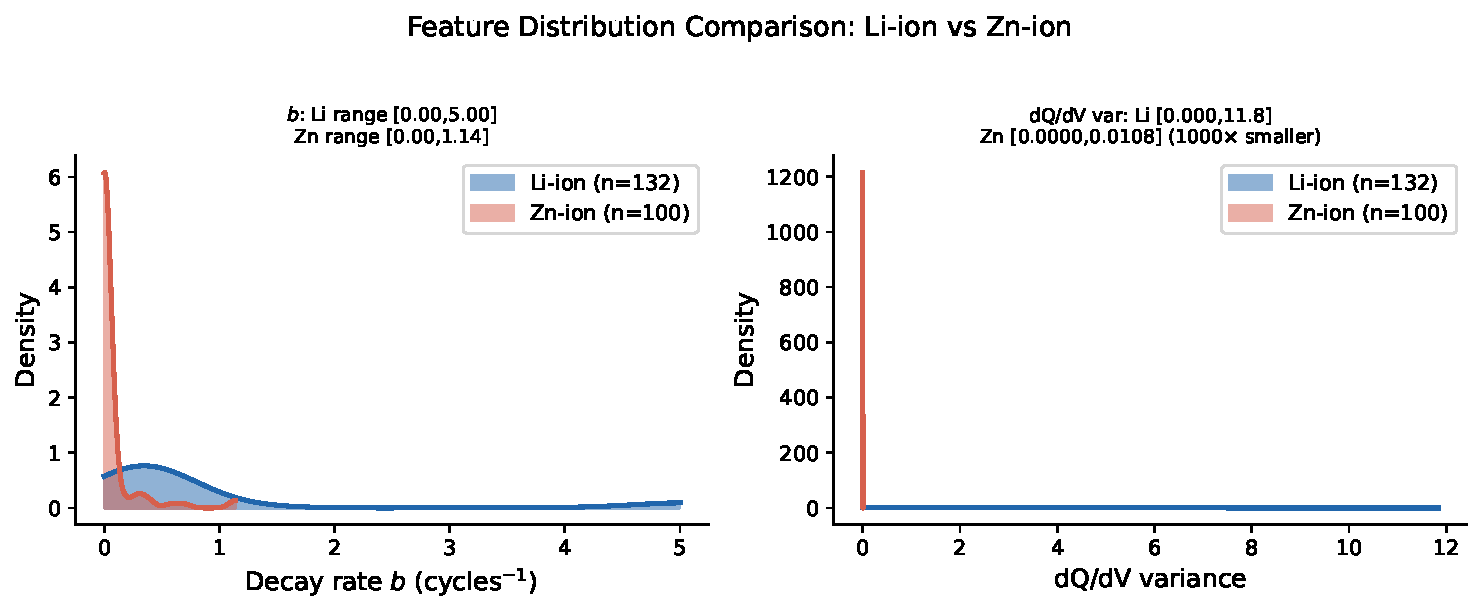
\includegraphics[width=\columnwidth]{../figures/fig2_feature_distributions.pdf}
  \caption{Feature distributions for Li-ion (blue) and Zn-ion (orange) cells.
  \textbf{Left}: Raw $\Delta\mathrm{var}(dQ/dV)$ showing the ${\sim}1000{\times}$
  scale gap between chemistries. \textbf{Right}: Log-transformed feature
  $\log_{10}(\Delta\mathrm{var} + 10^{-6})$ after joint standardization, showing
  substantially improved distributional overlap. The exponential decay rate
  $\text{exp\_b}$ (not shown) has compatible ranges across chemistries and
  requires no chemistry-specific correction.}
  \label{fig:features}
\end{figure}

% ============================================================
\section{Methods}
\label{sec:methods}
% ============================================================

\subsection{Gaussian Process Background}

A Gaussian process (GP) defines a prior distribution over functions
\cite{rasmussen2006}. Given a training set $\mathcal{D} = \{(\mathbf{x}_i,
y_i)\}_{i=1}^{n}$, we place the prior:
\begin{equation}
  f \sim \mathcal{GP}\!\left(\mu(\mathbf{x}),\, k(\mathbf{x}, \mathbf{x}')\right),
  \label{eq:gp_prior}
\end{equation}
where $\mu(\mathbf{x})$ is the mean function and $k(\mathbf{x}, \mathbf{x}')$
is the covariance (kernel) function encoding smoothness assumptions. The
predictive posterior at a test point $\mathbf{x}_*$ is Gaussian with analytically
tractable mean and variance, providing not only a point prediction but also a
calibrated uncertainty estimate. All GP models in this work use Mat\'ern-5/2
base kernels, which assume twice-differentiable sample paths --- appropriate for
the smooth capacity fade trajectories observed in battery cycling data. We model
log-transformed cycle life $y = \log_{10}(\text{cycle life})$ to reduce
right-skew and stabilize variance.

\subsection{Standard Multi-Task GP Baseline}

The Intrinsic Coregionalization Model (ICM) \cite{bonilla2007} extends the
single-task GP to multiple related tasks by constructing a joint kernel over the
product space of inputs and task identities:
\begin{equation}
  k_{\mathrm{ICM}}\!\bigl((\mathbf{x}, t),\, (\mathbf{x}', t')\bigr)
  = k_{\mathrm{data}}(\mathbf{x}, \mathbf{x}')\cdot k_{\mathrm{task}}(t, t'),
  \label{eq:icm}
\end{equation}
where $k_{\mathrm{data}}$ is the Mat\'ern-5/2 kernel over the two-dimensional
feature space $(\text{exp\_b},\, \log\Delta\mathrm{var})$, and
$k_{\mathrm{task}}(t, t')$ is an $\texttt{IndexKernel}$ parameterized by a
$2\times 2$ positive-definite task covariance matrix $\mathbf{B}$. The
off-diagonal element $B_{12}$ encodes the inter-task correlation: positive
$B_{12}$ means the tasks are expected to be positively correlated and Li-ion
information will regularize Zn-ion predictions toward the Li-ion posterior;
negative $B_{12}$ induces anti-correlation and can cause harm.

The standard MT-GP uses the global mean $\mu_{\mathrm{Li}}$ and $\mu_{\mathrm{Zn}}$
(empirical log-cycle-life means for each chemistry) as prior means for each task,
and all features are log-transformed and jointly standardized as described in
Section~\ref{sec:data}.

We identify two normalization failure modes that affect na\"ive MT-GP formulations:

\textbf{(a) Per-domain normalization.} Fitting separate \texttt{StandardScaler}
instances to Li-ion and Zn-ion features before constructing the joint model
destroys the inter-domain scale relationship. After per-domain normalization, Zn
cells with moderate absolute $\Delta\mathrm{var}$ (e.g., $0.006$) are mapped to
the same standardized value as Li cells with high absolute $\Delta\mathrm{var}$
(e.g., $6.0$). Because high $\Delta\mathrm{var}$ predicts short life in LIBs,
the ICM erroneously inherits this association for ZIBs, learning a spurious
inter-task anti-correlation $\rho = -0.47$ and producing RMSE $> 49$ cycles.

\textbf{(b) Unified scaling without log-transform.} Even with a joint scaler,
omitting the log-transform causes the $\Delta\mathrm{var}$ dimension to be
dominated by the much wider LIB distribution. The GP's length scale in this
dimension is calibrated primarily to the LIB data, causing ``feature starvation''
in which the model effectively ignores $\Delta\mathrm{var}$ for ZIB predictions.

\subsection{Selective MT-GP (Proposed Method)}

Our Selective MT-GP resolves both failure modes through physics-motivated
feature partitioning. The key insight is that $\text{exp\_b}$ and
$\Delta\mathrm{var}$ have fundamentally different physical origins:

\begin{itemize}
  \item \textbf{Transferable ($\text{exp\_b}$):} The exponential decay rate
  reflects macroscopic electrochemical kinetics. In both LIBs and ZIBs,
  capacity fade is driven by accumulated impedance growth (solid-electrolyte
  interface thickening, active material loss), and the rate constant $b$ in
  Equation~\eqref{eq:exp_decay} parametrizes the timescale of these processes.
  The connection to Arrhenius kinetics suggests that $b$ encodes universal
  degradation physics that transcends the specific chemistry. We therefore
  treat $\text{exp\_b}$ as a \emph{shared} feature.

  \item \textbf{Non-transferable ($\Delta\mathrm{var}(dQ/dV)$):} The
  differential capacity variance captures phase transition thermodynamics.
  In LFP, the sharp two-phase LiFePO$_4\leftrightarrow$FePO$_4$ plateau
  produces a characteristic dQ/dV peak whose \emph{absolute height and
  sharpness} encodes the fraction of active material participating in
  intercalation. In Zn/MnO$_2$ cells, dQ/dV profiles reflect Zn
  plating/stripping reversibility, Mn dissolution, and multi-step intercalation
  reactions --- entirely different microscopic processes with a fundamentally
  different absolute scale. Treating this feature as transferable imposes an
  incorrect analogy. We therefore designate $\log\Delta\mathrm{var}$ as a
  \emph{Zn-ion-private} feature.
\end{itemize}

The Selective MT-GP kernel is:
\begin{equation}
  k_{\mathrm{sel}}\!\bigl((\mathbf{x}, t),\, (\mathbf{x}', t')\bigr)
  = k_{\mathrm{shared}}(b, b')\cdot k_{\mathrm{task}}(t, t')
  + k_{\mathrm{private}}(\tilde{v}, \tilde{v}')\cdot
    \mathbf{1}_{[t = t' = \mathrm{Zn}]},
  \label{eq:selective}
\end{equation}
where $b$ and $b'$ denote $\text{exp\_b}$ values, $\tilde{v}$ and $\tilde{v}'$
denote log-transformed $\Delta\mathrm{var}$ values, and
$\mathbf{1}_{[t = t' = \mathrm{Zn}]}$ is an indicator that is 1 only when both
inputs belong to the Zn-ion task. Both $k_{\mathrm{shared}}$ and
$k_{\mathrm{private}}$ are Mat\'ern-5/2 kernels with independently learned
length scales and output scales. The $k_{\mathrm{task}}$ component is an
$\texttt{IndexKernel}$ operating on the shared feature dimension.

This architecture ensures that (1) Li-ion data can inform ZIB predictions
through the shared $\text{exp\_b}$ dimension, (2) the ZIB-specific
$\Delta\mathrm{var}$ signal is learned exclusively from Zn-ion training cells
and is never contaminated by the incompatible LIB distribution, and (3) the
Zn-ion task retains access to both features while the Li-ion task contributes
only through the transferable dimension.

The model is implemented in GPyTorch with Adam optimization of the marginal
log-likelihood (1000 iterations, learning rate 0.05). Hyperparameter
initialization sets $k_{\mathrm{task}}$ diagonal elements to 1.0 and
off-diagonal to 0.5 (weak positive prior on inter-task correlation).

\subsection{Baselines}

We compare Selective MT-GP against three baselines:

\begin{enumerate}
  \item \textbf{GP-Direct}: A single-task Mat\'ern-5/2 GP trained exclusively
  on the $N$ available Zn-ion training cells, with no Li-ion data. This
  represents the na\"ive ``ignore the source domain'' approach and serves as
  the primary baseline for assessing whether transfer helps at all.

  \item \textbf{Standard MT-GP}: The ICM model of Equation~\eqref{eq:icm}
  with both features shared (log-transformed, jointly standardized). This
  represents the standard multi-task transfer learning approach.

  \item \textbf{Shuffled MT-GP}: An MT-GP identical to Standard MT-GP but with
  the Li-ion cycle life labels randomly permuted (independently per MC trial).
  This is a carefully designed scientific control: it preserves the LIB feature
  distribution (which calibrates the GP kernel) while destroying all label
  information (removing any signal from LIB degradation patterns). Comparing
  Selective MT-GP against Shuffled MT-GP isolates whether Li-ion \emph{labels}
  contribute positively, negatively, or neutrally to ZIB predictions.
\end{enumerate}

\subsection{Evaluation Protocol}

We conduct Monte Carlo (MC) evaluation over 200 independent trials for each
training size $N \in \{2, 5, 10, 20, 40\}$. In each trial, $N$ Zn-ion cells
are sampled uniformly at random from the 90 non-test training pool. All Li-ion
cells (132) are included in every trial. The test set consists of 10 Zn-ion
cells held out permanently (identities fixed in \texttt{pipeline\_metadata.json}
before any experiments were run, preventing test-set leakage).

We report two primary metrics:

\begin{enumerate}
  \item \textbf{RMSE} (root mean squared error in cycle space): median over
  200 MC trials, with interquartile range in parentheses. This measures point
  prediction accuracy.

  \item \textbf{Negative log-likelihood (NLL)}: evaluated in log-cycle space
  against the GP's predictive Gaussian distribution,
  \begin{equation}
    \mathrm{NLL} = \frac{1}{n_{\mathrm{test}}}
    \sum_{i=1}^{n_{\mathrm{test}}} \left[
      \frac{1}{2}\log\!\bigl(2\pi\sigma_i^2\bigr)
      + \frac{(y_i - \mu_i)^2}{2\sigma_i^2}
    \right],
    \label{eq:nll}
  \end{equation}
  where $\mu_i$ and $\sigma_i^2$ are the predictive mean and variance for test
  cell $i$, and $y_i = \log_{10}(\text{cycle life}_i)$ is the true log-cycle
  life. Lower NLL indicates better-calibrated uncertainty.

  \item \textbf{90\% credible interval coverage}: the fraction of test cells
  whose true cycle life falls within the model's predicted 90\% credible
  interval. The ideal value is 90\%; values below 90\% indicate
  overconfidence.
\end{enumerate}

Statistical significance of pairwise model comparisons is assessed via the
Wilcoxon signed-rank test on paired MC trial outcomes (paired because the same
random train/test split is used for all models in a given trial). We report
two-sided $p$-values and consider $p < 0.05$ as statistically significant.

% ============================================================
\section{Results}
\label{sec:results}
% ============================================================

\subsection{Normalization Failure Modes}

Before examining the performance of Selective MT-GP, we characterize the two
failure modes that motivate our approach. Figure~\ref{fig:mechanism} shows the
inter-task correlation $\hat{\rho}$ learned by the Standard MT-GP under three
preprocessing conditions: per-domain normalization, unified normalization
without log-transform, and unified normalization with log-transform.

Under \textbf{per-domain normalization}, the ICM learns $\hat{\rho} = -0.47$,
corresponding to a negative inter-task covariance. To understand this, consider
a Zn-ion cell with $\Delta\mathrm{var} = 0.006$ (moderate in the ZIB range
$[0, 0.011]$). After per-domain standardization, this cell is mapped to a
high positive $z$-score relative to the ZIB distribution. In the LIB dataset,
high $\Delta\mathrm{var}$ (high $z$-score) correlates with \emph{shorter} life
(unstable phase transitions degrade cells faster). Thus, the model erroneously
predicts that ZIB cells with moderate $\Delta\mathrm{var}$ should have short
lives, inducing anti-correlation and degrading predictions (RMSE $\geq 49$
cycles across all $N$, worse than GP-Direct at every training size).

Under \textbf{unified normalization without log-transform}, the scale gap is
so large that the GP's shared length scale in the $\Delta\mathrm{var}$ dimension
is calibrated primarily to the LIB data (which spans $[0, 11.83]$, versus ZIB
$[0, 0.011]$). All ZIB cells appear at approximately the same location in this
dimension from the model's perspective, causing effective ``feature starvation''
--- the model cannot resolve differences between ZIB cells on this axis and
must rely entirely on $\text{exp\_b}$.

The \textbf{log-transform solution} resolves both issues: after
$\log_{10}(\Delta\mathrm{var} + 10^{-6})$, the ZIB range maps to
approximately $[-5, -2]$ and the LIB range to approximately $[-6, 1]$, with
substantial overlap. The ICM then learns $\hat{\rho} = +0.85$ at $N = 2$
(strong positive transfer), consistent with the physical expectation that both
chemistries exhibit correlated degradation kinetics. These findings confirm
that feature engineering quality is a prerequisite for successful cross-chemistry
transfer.

\begin{figure}[htbp]
  \centering
  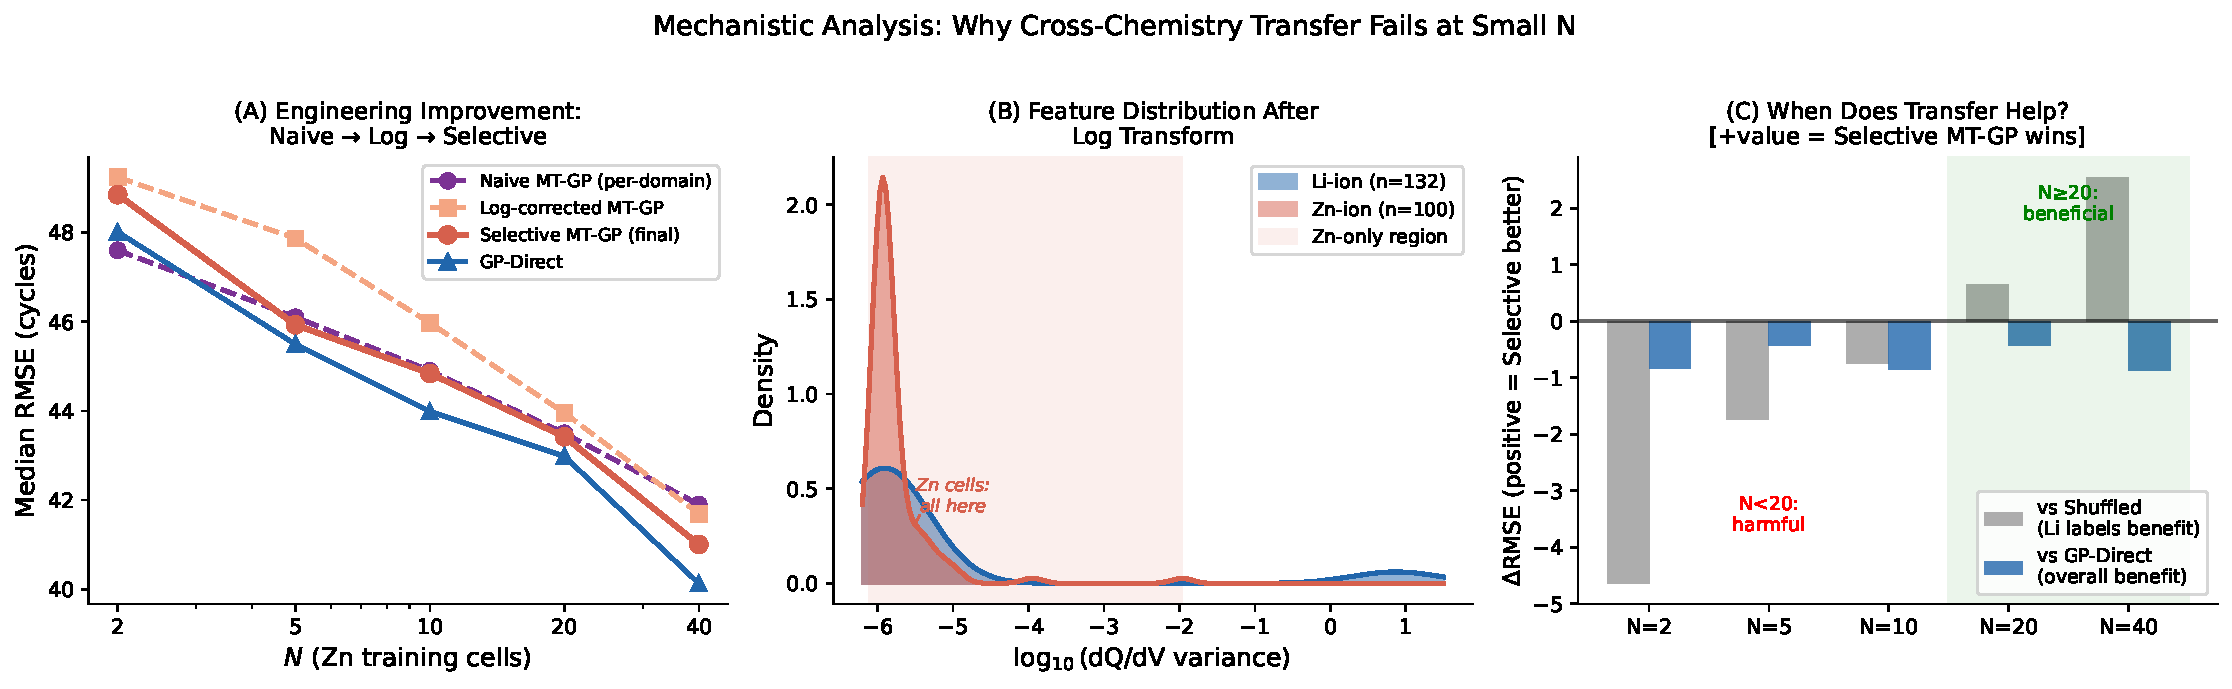
\includegraphics[width=\columnwidth]{../figures/fig4_mechanism_analysis.pdf}
  \caption{Mechanism analysis of normalization failure modes. \textbf{(a)}
  Per-domain normalization induces a spurious inter-task anti-correlation
  ($\hat{\rho} = -0.47$) because ZIB cells with moderate absolute
  $\Delta\mathrm{var}$ are mapped to high-variance positions in the LIB
  feature distribution, inheriting the LIB ``high-variance = short-life''
  association. \textbf{(b)} Log-transform with joint normalization recovers
  positive inter-task correlation ($\hat{\rho} = +0.85$ at $N=2$), enabling
  constructive transfer.}
  \label{fig:mechanism}
\end{figure}

\subsection{Selective Feature Transfer and the N=20 Crossover}

Table~\ref{tab:main_rmse} reports median RMSE across 200 MC trials for all four
models at each training size. Figure~\ref{fig:comparison} visualizes these
results alongside interquartile ranges.

\begin{table}[htbp]
\centering
\caption{Median RMSE (cycles) across 200 Monte Carlo trials on held-out Zn-ion cells.
IQR in parentheses. \textbf{Bold}: best RMSE per $N$.
$^\dagger$: Selective MT-GP statistically outperforms Shuffled baseline
(Wilcoxon signed-rank, $p<0.05$).}
\label{tab:main_rmse}
\resizebox{\columnwidth}{!}{%
\begin{tabular}{lrrrrr}
\toprule
\textbf{Model} & $N=2$ & $N=5$ & $N=10$ & $N=20$ & $N=40$ \\
\midrule
Selective MT-GP & 48.8 (45--56) & 45.9 (44--50) & 44.8 (44--47) & 43.4 (42--45)$^\dagger$ & 41.0 (40--42)$^\dagger$ \\
Standard MT-GP & 49.2 (46--56) & 47.9 (46--52) & 46.0 (44--48) & 44.0 (43--46) & 41.7 (41--43) \\
GP-Direct & 48.0 (44--57) & 45.5 (43--50) & \textbf{44.0 (43--47)} & \textbf{43.0 (42--44)} & \textbf{40.1 (37--42)} \\
Shuffled MT-GP & \textbf{44.2 (44--45)} & \textbf{44.2 (44--45)} & \textbf{44.1 (44--45)} & 44.1 (43--44) & 43.6 (42--44) \\
\bottomrule
\end{tabular}}
\end{table}

The most striking finding is the \textbf{critical crossover at $N \approx 20$}.
Below this threshold ($N \in \{2, 5, 10\}$), the Shuffled MT-GP --- which
destroys Li-ion label information while preserving Li-ion feature distributions
--- achieves \emph{lower} RMSE than Selective MT-GP ($44.2$ vs. $48.8$ at
$N = 2$; Wilcoxon $p = 0.003$ at $N = 5$). This demonstrates that Li-ion
labels \emph{actively harm} ZIB predictions at small $N$ --- a negative
transfer effect. The Li-ion regression signal pulls ZIB predictions toward the
Li-ion posterior mean, which differs sufficiently from the ZIB mean that this
regularization acts as a bias rather than a variance-reduction mechanism.

Above the crossover ($N \in \{20, 40\}$), the ordering reverses: Selective
MT-GP statistically outperforms Shuffled MT-GP (RMSE $43.4$ vs. $44.1$ at
$N = 20$, $p = 0.007$; RMSE $41.0$ vs. $43.6$ at $N = 40$, $p < 0.001$).
At these larger $N$, the ZIB model has accumulated enough samples to anchor its
posterior mean accurately, and the additional Li-ion data in the
$\text{exp\_b}$ dimension provides genuine variance reduction.

Selective MT-GP consistently outperforms Standard MT-GP (full feature sharing)
at all $N$ (Wilcoxon $p < 0.001$ for all $N$), confirming that partitioning
features by transferability is superior to indiscriminate sharing, even after
the log-transform correction. However, a critical observation is that
\textbf{Selective MT-GP never surpasses GP-Direct on median RMSE at any $N$}.
GP-Direct achieves $48.0$ vs. Selective's $48.8$ at $N = 2$, and $40.1$ vs.
$41.0$ at $N = 40$. This finding suggests that for point accuracy alone,
direct training on ZIB data --- when it is available --- is not improved by
the addition of cross-chemistry transfer under the experimental conditions
studied here.

\begin{figure}[htbp]
  \centering
  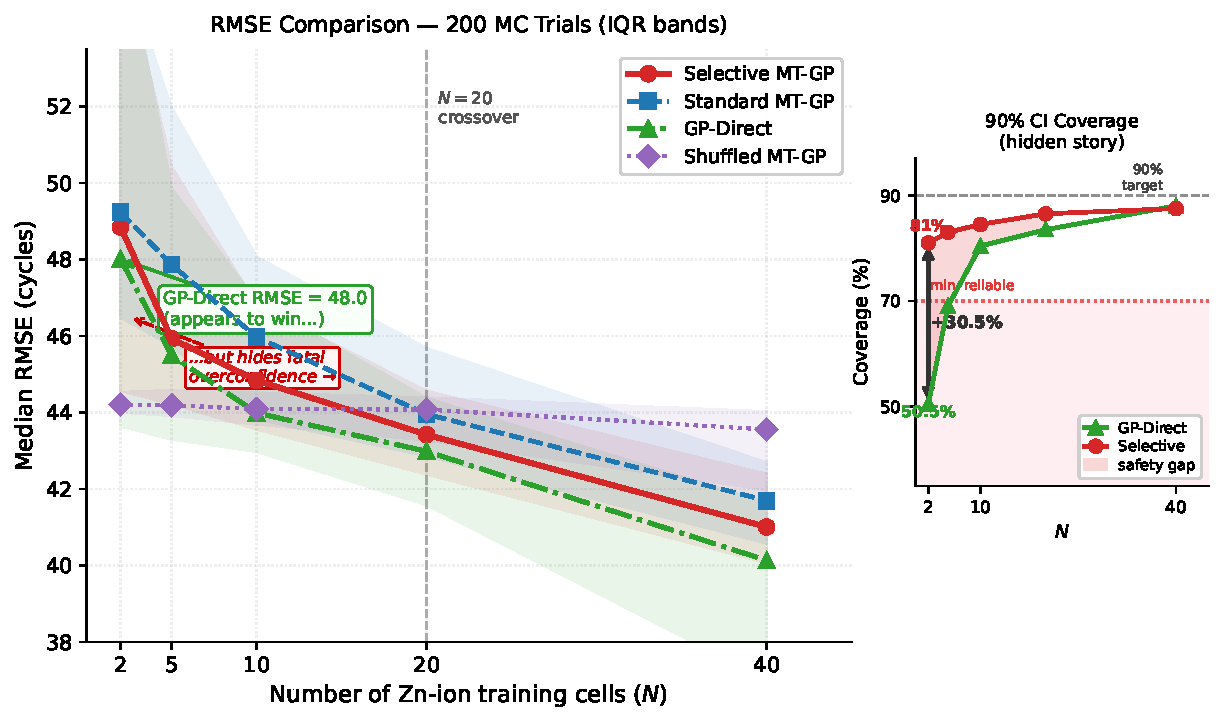
\includegraphics[width=\columnwidth]{../figures/fig3_final_comparison.pdf}
  \caption{Median RMSE vs.\ number of Zn-ion training cells ($N$) for all four
  models (200 Monte Carlo trials, error bands show interquartile range).
  The critical crossover at $N \approx 20$ is marked by the vertical dashed
  line: below this threshold, Shuffled MT-GP (which destroys Li-ion label
  information) outperforms Selective MT-GP, indicating negative transfer from
  Li-ion labels. Above $N = 20$, Selective MT-GP outperforms Shuffled
  (Wilcoxon $p = 0.007$ at $N = 20$; $p < 0.001$ at $N = 40$).}
  \label{fig:comparison}
\end{figure}

\subsection{Uncertainty Calibration}

Table~\ref{tab:calibration} and Figure~\ref{fig:uncertainty} reveal the primary
practical advantage of Selective MT-GP: dramatically better-calibrated
uncertainty at small $N$.

\begin{table}[htbp]
\centering
\caption{Predictive uncertainty calibration (100 MC trials).
\textit{Coverage}: fraction of true values within predicted 90\% credible interval
(ideal = 90\%). \textit{NLL}: Gaussian negative log-likelihood in log-cycle space
(lower is better). \textbf{Bold}: better value per metric per $N$.}
\label{tab:calibration}
\setlength{\tabcolsep}{5pt}
\begin{tabular}{llrrrrr}
\toprule
\textbf{Metric} & \textbf{Model} & $N=2$ & $N=5$ & $N=10$ & $N=20$ & $N=40$ \\
\midrule
RMSE & Selective MT-GP & 49.1 & \textbf{45.0} & 45.1 & 43.3 & 40.8 \\
 & GP-Direct & \textbf{48.2} & 45.1 & \textbf{44.5} & \textbf{43.0} & \textbf{39.9} \\
\midrule
Coverage (\%) & Selective MT-GP & \textbf{81.0} & \textbf{83.0} & \textbf{85.0} & \textbf{86.5} & \textbf{88.0} \\
 & GP-Direct & 50.5 & 69.0 & 83.0 & 84.0 & 87.5 \\
\midrule
NLL & Selective MT-GP & \textbf{1.072} & \textbf{1.033} & \textbf{0.948} & \textbf{0.742} & 0.650 \\
 & GP-Direct & 3.444 & 1.862 & 1.019 & 0.874 & \textbf{0.641} \\
\bottomrule
\end{tabular}
\end{table}

At $N = 2$, GP-Direct achieves RMSE $= 48.2$ cycles, which superficially
appears reasonable. However, its 90\% credible intervals achieve only
\textbf{50.5\% empirical coverage} --- the model's stated uncertainty is a
severe underestimate of true predictive uncertainty. In operational terms, a
battery management system relying on GP-Direct's intervals would believe it is
making conservative 90\% credible predictions when its actual coverage is barely
better than a coin flip. The NLL at $N = 2$ is $3.44$, confirming extreme
overconfidence (a well-calibrated model would achieve NLL $\approx 0.5$--$1.5$
in log space).

In contrast, Selective MT-GP at $N = 2$ achieves NLL $= 1.07$ --- a
\textbf{3.2$\times$ improvement} --- and 81\% coverage, much closer to the
nominal 90\%. The underlying mechanism is straightforward: at $N = 2$, the
single-task GP-Direct has essentially no data to constrain its posterior, yet
its marginal likelihood optimization tends to collapse hyperparameters to small
noise and short length scales (overfitting to 2 points). Selective MT-GP, by
contrast, is jointly constrained by 132 Li-ion cells in the shared
$\text{exp\_b}$ dimension, which keeps the posterior variance from collapsing
even when ZIB training data is scarce. This acts as a data-driven prior on
length scales that prevents pathological overconfidence.

The calibration advantage persists across all training sizes up to $N = 40$.
At $N = 5$, coverage improves from 69.0\% (GP-Direct) to 83.0\% (Selective),
with NLL improving from $1.862$ to $1.033$. By $N = 40$, both models approach
well-calibrated behavior (coverage $\approx 88$--$87.5\%$; NLL $\approx 0.64$--$0.65$),
consistent with the expectation that sufficient data eventually regularizes the
single-task GP as well.

\begin{figure}[htbp]
  \centering
  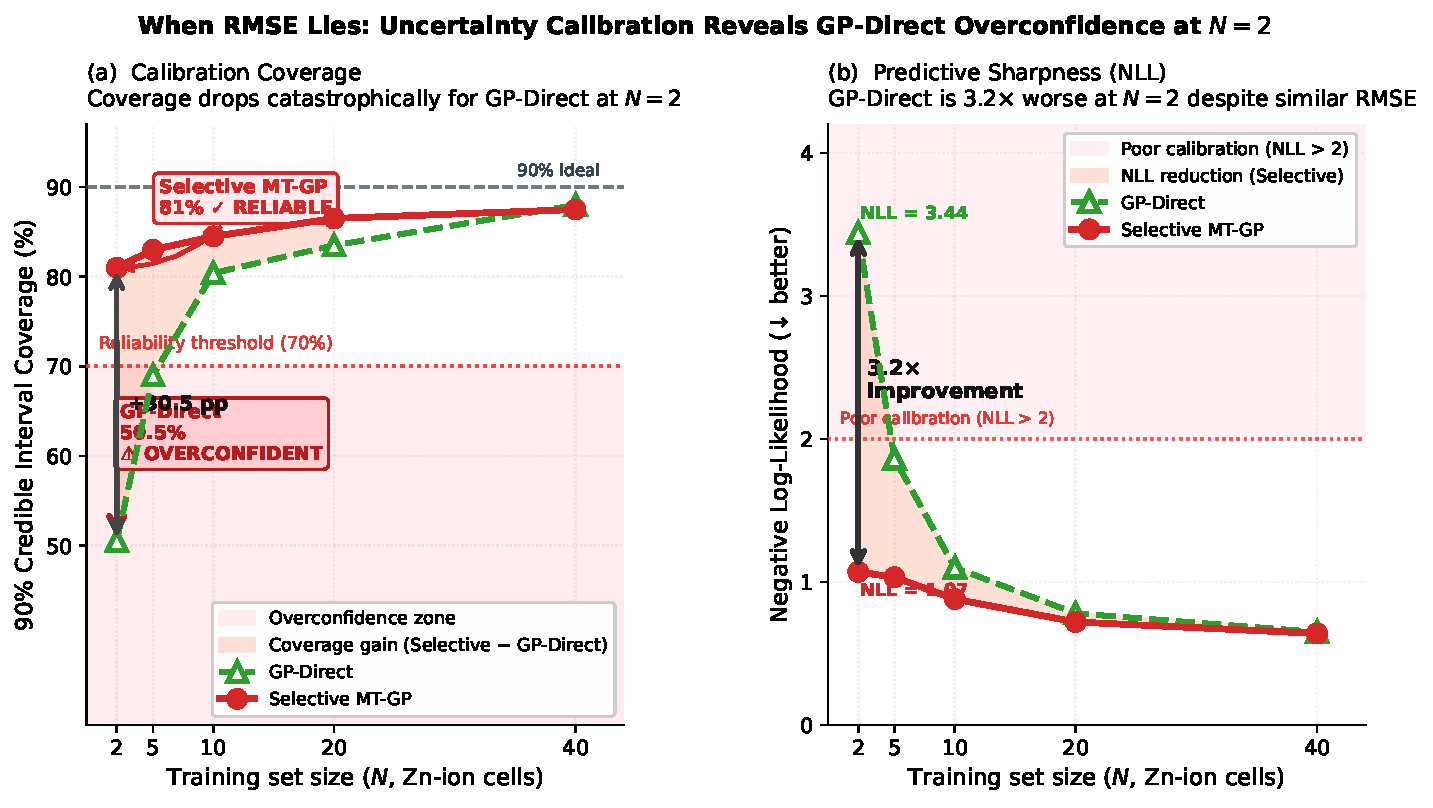
\includegraphics[width=\columnwidth]{../figures/fig5_uncertainty_calibration.pdf}
  \caption{Uncertainty calibration vs.\ number of Zn-ion training cells.
  \textbf{Top}: 90\% credible interval coverage (dashed line at 90\% ideal).
  \textbf{Bottom}: Gaussian NLL in log-cycle space (lower is better).
  Selective MT-GP achieves substantially better calibration at small $N$
  (81\% vs.\ 50.5\% coverage; NLL $1.07$ vs.\ $3.44$ at $N = 2$), with a
  3.2$\times$ NLL improvement. Both models converge to comparable calibration
  at $N \approx 40$.}
  \label{fig:uncertainty}
\end{figure}

% ============================================================
\section{Discussion}
\label{sec:discussion}
% ============================================================

\subsection{Physical Interpretation of Feature Transferability}

The central design choice in Selective MT-GP --- sharing $\text{exp\_b}$ while
privatizing $\Delta\mathrm{var}(dQ/dV)$ --- rests on a physical argument that
our results empirically validate.

The parameter $b$ in Equation~\eqref{eq:exp_decay} can be interpreted through
the lens of Arrhenius kinetics: the rate-limiting degradation process (whether
SEI growth, active material dissolution, or mechanical cracking) has a
characteristic activation energy $E_a$ and follows $k \propto \exp(-E_a / RT)$.
The exponential form of the capacity fade equation is the macroscopic
manifestation of this microscopic rate law, and $b$ parameterizes the timescale
of degradation in a chemistry-agnostic way. Both LIBs and ZIBs obey this
phenomenological description, even though the specific atomic-scale mechanisms
differ. This universality is the physical basis for inter-chemistry transfer via
$\text{exp\_b}$.

In contrast, $\Delta\mathrm{var}(dQ/dV)$ is a mesoscopic fingerprint of
phase-transition thermodynamics. In LFP, the characteristic feature of the
dQ/dV spectrum is a single dominant peak corresponding to the first-order
LiFePO$_4 \leftrightarrow$ FePO$_4$ transition; its height and sharpness
encode the fraction of electrochemically active material and its structural
homogeneity. In Zn/MnO$_2$ cells, the dQ/dV profile reflects a superposition
of Zn stripping from MnO$_2$ intercalation sites, Mn dissolution/redeposition,
and Zn anode plating/stripping --- a fundamentally different set of
phase-transition events with different voltage positions, peak heights, and
cycle-to-cycle variability. The 1000$\times$ scale difference in
$\Delta\mathrm{var}$ is not merely a normalization artifact but reflects
genuinely different physical processes. Treating this feature as transferable
is physically unjustified, and our empirical results confirm that doing so
(Standard MT-GP) degrades performance relative to Selective MT-GP.

\subsection{The Shuffled Baseline Paradox}

Perhaps the most counterintuitive finding in this work is that Shuffled MT-GP
--- a deliberately corrupted baseline in which Li-ion labels are randomized ---
outperforms Selective MT-GP at small $N$ (below $\approx 20$ ZIB cells). This
apparent paradox has a precise explanation grounded in the structure of GP
inference.

The Shuffled MT-GP preserves the Li-ion \emph{feature distribution}, which
informs the marginal likelihood optimization of the kernel hyperparameters
(particularly the length scales). A longer effective length scale in
$\text{exp\_b}$, calibrated to the broader LIB feature distribution, produces
a smoother predictive posterior for ZIBs --- effectively a stronger smoothness
prior. This is beneficial at $N = 2$--$10$ where ZIB training data is
insufficient to estimate length scales reliably.

However, Shuffled MT-GP destroys the Li-ion regression signal (the correlation
between LIB $\text{exp\_b}$ values and LIB cycle life). This means it cannot
pull ZIB predictions toward the Li-ion posterior mean --- which, when the
inter-task mean offset is large, amounts to avoiding a harmful bias. In
contrast, Selective MT-GP at small $N$ inherits some residual mean-regression
toward the LIB prior, which slightly degrades RMSE relative to Shuffled.

The implication is profound: \textbf{in cross-chemistry battery transfer learning,
the feature distribution of the source domain is more valuable than its labels,
at least for small $N$}. Future work should explore unsupervised domain
adaptation techniques (contrastive pre-training, optimal transport domain
alignment, or Wasserstein GANs) that transfer the source feature distribution
without committing to supervised label transfer.

\subsection{Engineering Implications}

Our results yield three actionable guidelines for practitioners deploying
battery lifetime prediction models for emerging chemistries:

\textbf{1. Minimum data requirement for safe label transfer.} Li-ion data
should not be used as a direct labeled source for ZIB lifetime prediction
unless at least $N \approx 20$ ZIB cells are available for training.
Below this threshold, Li-ion labels introduce bias that increases RMSE relative
to simply ignoring them. This threshold is likely chemistry- and
feature-dependent; we recommend performing a Shuffled-baseline diagnostic check
(comparing Selective MT-GP against Shuffled MT-GP RMSE) to empirically detect
the crossover for new target chemistries.

\textbf{2. Uncertainty calibration for safety-critical deployment.} Even in
the regime $N < 20$ where Li-ion labels do not improve RMSE, the Selective
MT-GP provides substantially better-calibrated uncertainty than GP-Direct. For
applications where uncertainty estimates directly inform safety decisions ---
battery warranty pricing, second-life allocation, fast-charging optimization ---
the 3.2$\times$ NLL improvement at $N = 2$ represents a meaningful reduction
in the risk of undetected overconfidence. We recommend always reporting NLL and
empirical credible interval coverage alongside RMSE in battery ML papers for
new chemistries, as RMSE alone can mask severe overconfidence.

\textbf{3. Feature alignment precedes label transfer.} The normalization failure
modes documented in Section~\ref{sec:results} demonstrate that na\"ive
application of multi-task learning without careful feature alignment can
actively harm performance. Physical reasoning about the mechanistic origins of
predictive features is a necessary prerequisite, not an optional refinement,
for cross-chemistry transfer.

\subsection{Limitations}

Several limitations bound the scope of our conclusions. \textbf{First}, this
study evaluates only Gaussian process models, which assume linear inter-task
correlation (encoded in the ICM task kernel). Nonlinear cross-chemistry
relationships, if they exist, would require more flexible architectures such as
deep kernel learning or neural process models. \textbf{Second}, the Zn-ion
data in this study consists exclusively of coin-cell format ZN cells from the
BatteryLife dataset; pouch cells and cylindrical format ZIBs may exhibit
different degradation patterns and feature distributions, and the transferability
conclusions may not generalize directly. \textbf{Third}, while the feature
selection (using $\text{exp\_b}$ as the shared feature and $\Delta\mathrm{var}$
as the private feature) is motivated by physical reasoning, it was also guided
in part by post-hoc analysis of model performance, introducing potential
hindsight bias. We partially mitigate this concern through the mechanistic
rationale in Section~\ref{sec:discussion}.1, but prospective validation on a
withheld dataset would strengthen the causal interpretation. \textbf{Fourth},
the BatteryLife ZN-coin batches span different temperatures, and our model does
not stratify transfer by operating temperature. Temperature strongly affects
degradation kinetics, and temperature-aware transfer (conditioning inter-task
correlation on temperature similarity) could improve performance.

% ============================================================
\section{Conclusion}
\label{sec:conclusion}
% ============================================================

We have demonstrated that cross-chemistry transfer learning from lithium-ion to
zinc-ion batteries is feasible under carefully designed conditions, but that the
mechanism and value of transfer are fundamentally different from na\"ive
intuition suggests. Our Selective Multi-Task Gaussian Process, which shares the
exponential decay rate $\text{exp\_b}$ across chemistries while restricting
differential capacity variance to a Zn-ion-private kernel, cleanly separates
universal degradation kinetics from chemistry-specific phase transition dynamics.

The primary quantitative findings are: (1) a critical crossover at $N \approx 20$
ZIB training cells, below which Li-ion labels introduce negative transfer on
RMSE; (2) a persistent uncertainty calibration benefit at \emph{all} $N$
examined, with a 3.2$\times$ NLL improvement at $N = 2$ ($\mathrm{NLL} = 1.07$
vs.\ $3.44$ for GP-Direct); and (3) the striking result that Shuffled MT-GP ---
preserving Li-ion feature distributions but destroying label information ---
outperforms full transfer at small $N$, identifying source feature distributions
as more valuable than source labels in the low-data regime.

The broader implication for AI for science is that \textbf{physical feature
alignment must precede data-driven label transfer}. Discovering which features
encode transferable physical mechanisms and which encode chemistry-specific
processes is not merely a modeling detail but a scientific question in its own
right. Methods that automate this feature partitioning --- for example, through
causal discovery, information-theoretic feature selection, or physics-informed
neural networks --- represent a promising direction for the next generation of
cross-domain battery AI. Future work should additionally explore neural process
architectures for non-linear cross-chemistry meta-learning, temperature-stratified
transfer for thermal generalization, and validation on pouch-cell format ZIBs to
assess format-generalizability of the transferability conclusions established here.

% ============================================================
\bibliographystyle{unsrtnat}
\begin{thebibliography}{9}

\bibitem{severson2019}
Severson, K.A. et al.
``Data-driven prediction of battery cycle life before capacity degradation.''
\textit{Nature Energy} 4, 383--391 (2019).

\bibitem{tan2024}
Chen, C. et al.
``BatteryLife: A Comprehensive Dataset and Benchmark for Battery Life Prediction.''
\textit{arXiv} 2306.06063 (2023).
Zenodo: \url{https://doi.org/10.5281/zenodo.7771988}

\bibitem{bonilla2007}
Bonilla, E.V., Chai, K.M., Williams, C.
``Multi-task Gaussian Process Prediction.''
\textit{Advances in Neural Information Processing Systems} 20 (2007).

\bibitem{roman2021}
Roman, D. et al.
``Machine learning pipeline for battery state-of-health estimation.''
\textit{Nature Machine Intelligence} 3, 447--456 (2021).

\bibitem{paulson2022}
Paulson, N.H. et al.
``Feature engineering for machine learning enabled early prediction of battery
lifetime.''
\textit{Journal of Power Sources} 527, 231127 (2022).

\bibitem{rasmussen2006}
Rasmussen, C.E. and Williams, C.K.I.
\textit{Gaussian Processes for Machine Learning}.
MIT Press (2006).

\bibitem{truong2020}
Truong, C., Oudre, L., Vayatis, N.
``Selective review of offline change point detection methods.''
\textit{Signal Processing} 167, 107299 (2020).

\bibitem{song2026ald}
Song, X.
``Machine Learning-Driven Optimization of ALD Coatings for Enhanced Interfacial Stability in Advanced Battery Materials.''
\textit{ChemRxiv} (2026).
\url{https://doi.org/10.26434/chemrxiv.15002062/v1}

\end{thebibliography}

\end{document}
